\chapter{Stand van zaken}
\label{ch:stand-van-zaken}

% Tip: Begin elk hoofdstuk met een paragraaf inleiding die beschrijft hoe
% dit hoofdstuk past binnen het geheel van de bachelorproef. Geef in het
% bijzonder aan wat de link is met het vorige en volgende hoofdstuk.

% Pas na deze inleidende paragraaf komt de eerste sectiehoofding.

Vooraleer er onderzoek gedaan wordt naar een oplossing voor examens op eigen computer moet er gekeken worden naar de huidige situatie op de Hogeschool Gent. Het is ook belangrijk te kijken wat er achter het buzzword BYOD zit en welke BYOD oplossingen er momenteel op de markt zijn. 
%Dit hoofdstuk bevat je literatuurstudie. De inhoud gaat verder op de inleiding, maar zal het onderwerp van de bachelorproef *diepgaand* uitspitten. De bedoeling is dat de lezer na lezing van dit hoofdstuk helemaal op de hoogte is van de huidige stand van zaken (state-of-the-art) in het onderzoeksdomein. Iemand die niet vertrouwd is met het onderwerp, weet er nu voldoende om de rest van het verhaal te kunnen volgen, zonder dat die er nog andere informatie moet over opzoeken \autocite{Pollefliet2011}.

\section{Examens op Hogeschool Gent}

\subsection{Soorten examens}
Op Hogeschool Gent, Faculteit Bedrijf en Organisatie worden er 2 soorten examens afgenomen, mondelinge en schriftelijke. Enkele schriftelijke examens worden enkel op papier afgelegd, anderen deels of volledig op computer. Dit zijn de soorten computerexamens die op Hogeschool Gent afgenomen worden:
\begin{itemize}
\item Een online test waarbij antwoorden via de webbrowser invgevuld worden (bv. via Chamilo, Cisco-platform, enz.)
\item Een schriftelijk examen waaarbij de voorbereiding op pc gebeurt maar de antwoorden op papier ingevuld worden.
\item Een examen dat op computer m.b.v. specifieke software (bv. IDE en compiler) gemaakt wordt waarna het resultaat digitaal ingediend wordt (bv. Word document met antwoorden, zip-bestand met broncode, Github, ...)
\end{itemize}


\subsubsection{Schriftelijke examens (deels op computer) }

De student heeft toegang tot software (vb. Netbeans, Microsoft Excel, Microsoft Word) en documenten (vb. Examenopgave, Microsoft PowerPoints, PDF-documenten) die zich lokaal bevinden, op vraag van de lector. Deze examens worden altijd op desktops van Hogeschool Gent afgenomen. In een beveiligde gemonitorde omgeving, waarin enkel toegelaten is wat toegestaan is door de lector. De examenopzichter heeft via de admin-computer zicht op alle bureaubladen van de studenten die het examen aan het afleggen zijn. 




\subsubsection{Schriftelijke examens (volledig op computer)}

\paragraph{Examens waarbij toegang tot het gehele systeem vereist is}

Met toegang tot het gehele systeem wordt er bedoeld dat de student hier ook toegang heeft tot software  en documenten die zich lokaal bevinden. Deze examens worden net zoals examens die deels op computer afgenomen worden, altijd op desktops van Hogeschool Gent afgenomen, in diezelfde beveiligde omgeving. Enkel moet de student zijn ingevulde examen digitaal indienen en worden eventuele notities op papier niet bekeken.  

\paragraph{Examens waarbij enkel toegang tot een webbrowser vereist is}

Wanneer er enkel toegang tot een webbrowser vereist is (Test op chamilo, Online-vragenlijst) hoeft het examen niet op een desktop van Hogeschool Gent afgelegd te worden. Dit kan ook gewoon via de browser op de laptop van een student. Dit brengt natuurlijk enkele risico's met zich mee. De lector heeft geen zicht op hetgeen de student doet en de student kan communiceren met medestudenten achter de rug van een opzichter. Er kunnen ook bepaalde problemen met de browser opduiken, zoals met plugins, browsertype of browserversie. 

\subsection{Huidige examensysteem}

\subsubsection{Omschrijving van het huidige systeem}
In het huidige systeem beschikt de Hogeschool Gent over een groot aantal windows machines. Op elke machine kan elk examen uitgevoerd worden. Dit houdt in dat er zo'n 180 softwarepaketten (over alle richtingen heen) onderhouden moeten worden door de systeembeheerders. Elke computer moet ook gelicensieerd zijn voor de NetSupport School software. Per computerlokaal staat er ook 1 admincomputer. Deze wordt gebruikt om studenten tijdens een examen te monitoren, om beperkingen voor de studenten in te stellen, om examendocumenten op de computer te plaatsen en ze na het examen terug af te halen. NetSupport school zorgt concreet voor een beveiligde en gemonitorde omgeving voor studenten om hun examen af te leggen. 



\begin{figure}
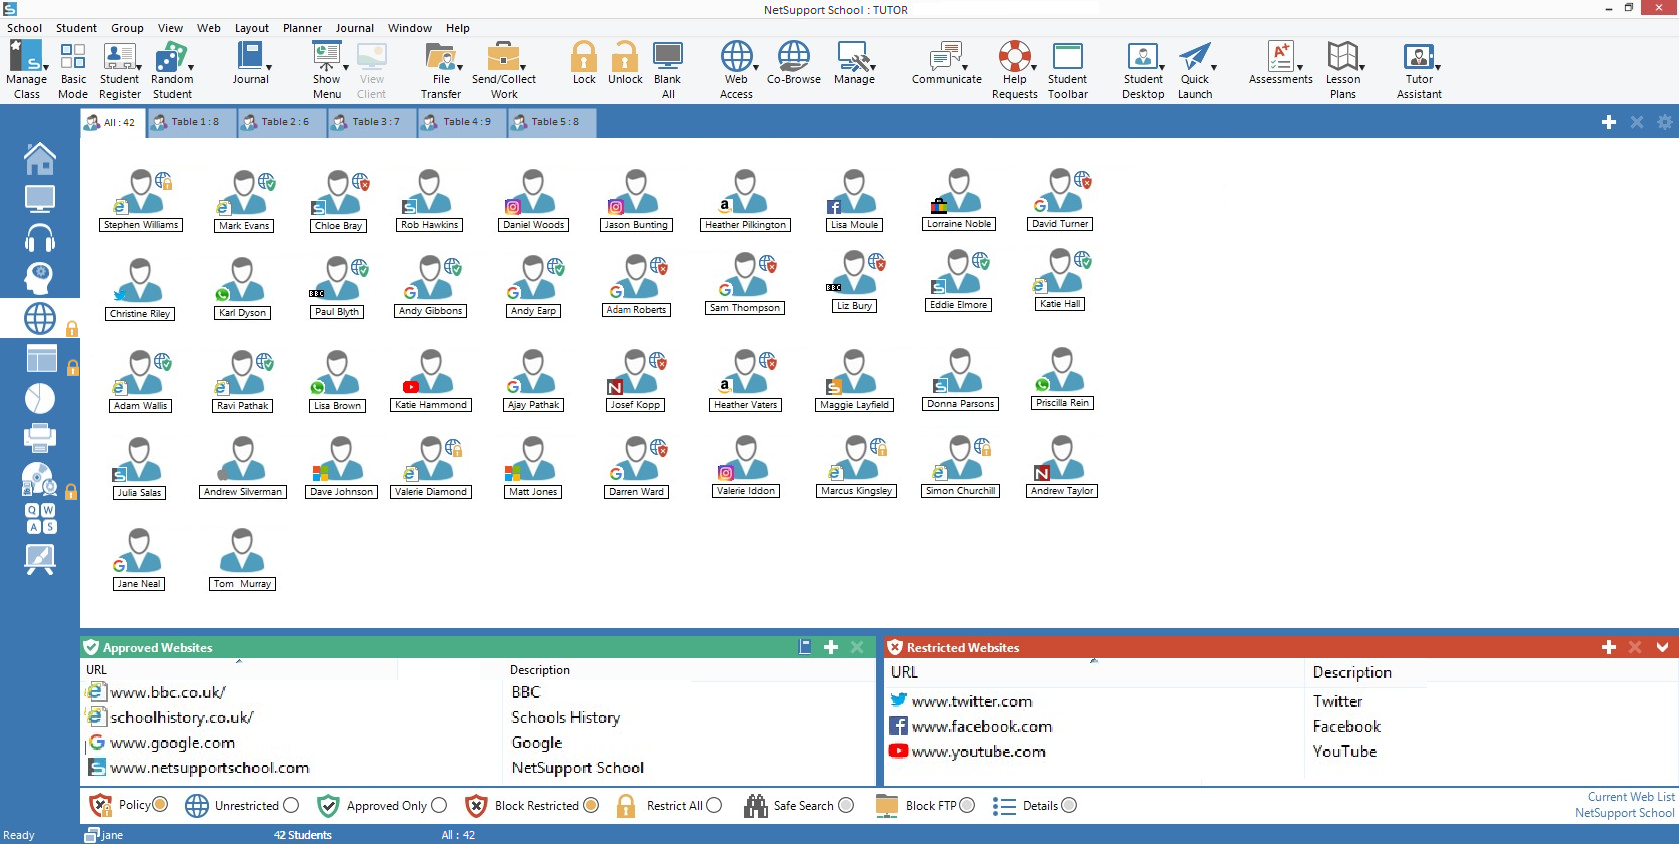
\includegraphics[width=\linewidth]{img/NetsupportAdmin.png}
\caption{Screenshot van het scherm op de admincomputer van een netsupport school-omgeving}
\label{fig:NetSupport1}
\end{figure}


\subsubsection{Tekortkomingen}


\paragraph{Tekortkomingen volgens een lector}

Deze paragraaf is gebaseerd op een interview met een lector. Het huidige systeem bevat volgens die lector meerdere tekortkomingen. De lectoren hebben te veel werk bij het actuele systeem. Ze moeten lang op voorhand doorgeven welk examen er wanneer zal doorgaan en welke software er daarvoor nodig is. Maar zelfs dan loopt het af en toe nog mis, cfr. examen webapplicaties III 2018-2019, toen moest dat examen tot het einde van de examenperiode uitgesteld worden omdat de verkeerde versie van de IDE geinstalleerd was.

Zelfs indien het klaarzetten van de software goed verloopt, moeten de lectoren toch nog extra werk doen. Op voorhand testen ze de omgeving, en op de dag van het examen zelf zijn ze tot 1.5 uur bezig voor de aanvang van het examen, om alle files op de juiste locatie te plaatsen met NetSupport School en om te controleren of dit overal gelukt is. De student krijgt tijdens het examen instructies om zijn examen correct in te dienen. Bijvoorbeeld: 'plaats het document met een bepaalde naam in een map met bepaalde naam.' Dit moet exact zijn en er is geen ruimte voor fouten (hoofd- of kleine letter, underscore of koppelteken). Volgens de lector loopt het digitaal ophalen van de examens in 5\% tot 7.5\% van de gevallen fout (Bij een klas van 40 studenten).
Dan moet er manueel ingegrepen worden op de computers om de benaming in orde te brengen. Na het afhalen van de examens moeten alle files die aangemaakt zijn door en voor de student ook nog eens verwijderd worden van de computer. Dit kan tot 3 uur tijd in beslag nemen na elk examen.  

Die Lector zou met het nieuwe examensysteem zeker het gebruik van internet moeten kunnen beheren en communicatie tussen studenten tegenhouden. Liefst van al zou ze ook de studenten verbieden om lokaal op hun laptop naar documenten te kijken. Het huidige systeem zou vooral gemoderniseerd moeten worden, waardoor de lectoren er minder werk aan hebben, en de studenten zelf verantwoordelijk zouden zijn voor het indienen van hun examen. 


\paragraph{Tekortkomingen volgens een systeembeheerder}
Hier volgen de problemen die een systeembeheerder van Hogeschool Gent aanhaalde. Volgens de systeembeheerder zijn de lectoren zijn niet genoeg opgeleid om met het NetSupport School-systeem te werken. Op die manier hebben veel lectoren te weinig inzicht in de werking van NetSupport School. Vaak zouden de fouten die voorkomen vermeden kunnen worden door extra opleidingen of ondersteuning. Dit geheel zorgt voor veel extra werk voor de lectoren en systeembeheerders. 

Aan de kant van het systeembeheer zijn er ook meerdere klachten. Het uitrollen van nieuwe softwarepaketten wordt niet gedaan door iemand die daar fulltime mee bezig is. Het schrijven van SCCM pakketten zou enkel door een ervaren iemand gedaan mogen worden.  Met het huidige systeen krijg je soms verkeerd geconfigureerde software op de dag van het examen en moeten examens uitgesteld worden. Er wordt te weinig getest. Fouten met software zouden vermeden moeten worden. 

\subsection{Vereisten voor een examensysteem}

Voor wer een nieuw examensysteem opgezet kan worden is het belangrijk om de vereisten hiervan in kaart te brengen. Hier alvast een lijst met mogelijke eigenschappen van een examensysteem: 
	\begin{itemize}
	\item Toegang tot het internet kan verboden worden.
	\item Beperken van toegang tot documenten.
	\item Beperken van toegang tot software.
	\item Digitale communicatie met medestudenten is niet mogelijk.
	\item Monitoring tijdens het examen.
	\item Snel en makkelijk opzetten van examens. 
	
\end{itemize}	

Uit deze lijst stellen via de MoSCoW-methode onze prioriteiten op. MoSCoW staat voor: must haves, should haves, could haves en won't haves. In samenspraak met de ge\"{i}nterviewden zijn de prioriteiten op deze manier vastgelegd. 

	\begin{itemize}
	\item Must haves
		\begin{itemize}
		\item Toegang tot het internet kan verboden worden.
		\item Digitale communicatie met medestudenten is niet mogelijk.
		\item Snel en makkelijk opzetten van examens. 
		\item Beperken van toegang tot documenten.
		
	\end{itemize}	
	\item Should haves
		\begin{itemize}
		\item Geen.
	
		
	\end{itemize}	
	\item Could haves
		\begin{itemize}
		\item Beperken van toegang tot software.
		\item Monitoring tijdens het examen.
		
	\end{itemize}	
	\item won't haves
		\begin{itemize}
		\item Geen.
		
	\end{itemize}	
	\end{itemize}	

Beperken van toegang tot documenten zou zowel bij must haves als shoud haves kunnen staan. Volgens een lector die computerexamens afneemt hangt het van examen tot examen af of toegang tot documenten beperkt moet worden. Vooral examens die afgelegd worden door eerstejaarsstudenten zouden volgens die lector zonder toegang tot alle mogelijke documenten op de laptop van de student afgenomen moeten kunnen worden. Aangezien het beperken van toegang tot documenten in sommige gevallen moet kunnen gebeuren, is er beslist om dit toch bij de must haves te plaatsen. 



\section{BYOD}

BYOD ofwel Bring Your Own Device is een term die de laatste jaren wel vaker opduikt. Door de overvloed van nieuwe apparaten en gadgets, die aan een rotvaart op de markt gebracht worden, is het voor vele bedrijven te duur om altijd mee te zijn met de meest actuele technologieën. De opkomst van BYOD zorgt voor een verschuiving van de overheadkosten, die het beheer van vele apparaten in het bedrijf met zich meebrengt, van het bedrijf naar de werknemers toe \autocite{Hong2016}.

\section{BYOD examens}
Bij BYOD examens leggen studenten examens af op hun eigen laptop. Deze manier van werken is nog niet wijdverspreid. Het kent enkele voor- en nadelen. In de volgende secties wordt hier verder over uitgeweid. 

\subsection{Voordelen van BYOD examens}
Het meest prominente voordeel dat BYOD examens met zich meebrengen is het feit dat studenten in een vertrouwde omgeving kunnen werken. Daardoor neemt hun stressgevoeligheid af, volgens
\textcite{TeckSwee2014}. In het onderzoek van \textcite{TeckSwee2014}, waarbij er na een BYOD examen gepolst werd naar de tevredenheid van de deelnemers, bleek 74.02\% van de ondervraagde leerlingen (672) meer tevreden te zijn met deze manier om examens af te nemen, in vergelijking met het afleggen van een examen op een computer van de onderwijsinstelling. 

Andere voordelen zijn belangrijker voor de onderwijsinstelling. Doordat de computers uit hun beheer gaan is er een kleinere overhead voor de systeembeheerders en een lagere kost voor de instelling.

\subsection{Opmerkingen bij BYOD examens}

Aangezien examens afleggen op eigen hardware een relatief nieuw gegeven is, ervaren we nog enkele kinderziektes. Die problemen kunnen we in 2 groepen indelen: veiligheid en werkbaarheid.\\ 

\subsubsection{Problemen op vlak van veiligheid}
Wanneer je niet de volledige controle over een apparaat hebt kan de mogelijkheid tot fraude niet altijd even makkelijk of zelfs niet vermeden worden.
\textcite{Dawson2016} bekeek in zijn onderzoek vijf manieren om fraude te plegen tijdens een examen op eigen laptop, waaronder de volgende drie belangrijkste worden opgesomd: 
\begin{itemize}
	\item De examenopgave lokaal opslaan en achteraf online plaatsen.
	\item Het examen in een virtuele omgeving afleggen en op die manier het besturingssysteem manipuleren
	\item Software aanpassingen maken 

\end{itemize}

Deze methodes zijn gerangschikt volgens de kans dat een student tijdens de beperkte examentijd \'{e}\'{e}n van deze methodes toepast.  

\textbf{De examenopgave lokaal opslaan en achteraf online plaatsen.} Als de student de examenopgave lokaal krijgt, weerhoudt hem niets om lokaal een kopie te maken en die achteraf (tegen betaling) te verspreiden. Dit zorgt er voor dat de meeste studenten de examens die het jaar ervoor gegeven zijn kunnen inkijken en oplossen of de oplossingen kunnen bekijken. In de snel veranderende wereld van Information Technology hoeft dit geen probleem te zijn, de leerstof kan per jaar genoeg vari\"{e}ren. Het betekent natuurlijk wel dat de student de vraagstelling of de soort oefeningen die op het examen zal voorkomen beter kan inschatten. Met dit gegeven zal rekeninng gehouden moeten worden bij het opstellen van examens die afgenomen worden op een apparaat van de student. 

\textbf{Het examen op een virtuele omgeving afleggen en op die manier het besturingssysteem manipuleren.} Wanneer er tijdens een computerexamen gemonitord zou worden op systeemvlak, kan een student makkelijk die monitoringsoftware installeren op een virtuele machine en dan op het hostsysteem niet gemonitorde acties uitvoeren (Opzoeken op het internet, communicatie via het internet, opzoeken in lokale documenten). Hierop kan enkel gecontroleerd worden door elke laptop af te gaan em zo te kijken of de software op de host zelf ge\"{i}nstalleerd is, maar zelfs deze methode is niet waterdicht. Je kan enkel zeker zijn dat de student niet met een virtuele machine werkt wanneer de instelling zelf de software zou installeren. Maar, als apparaten dan toch beheerd worden door de instelling zelf verlies je de voordelen van het BYOD-principe (minder overhead en minder kosten).

\textbf{Software aanpassingen maken.} Aangezien de student de software zelf beheert heeft hij de kans om de software aan te passen, zeker wanneer het open-source software betreft. Het is bijvoorbeeld mogelijk theorie of formules verstoppen in de broncode. De reden waarom dit zo laag op de lijst staat is omdat het voor een student veel makkelijker is om gewoon een cheat sheet als document te verstoppen op zijn laptop en zo theorie of formules te bekijken. 

\subsubsection{Problemen op vlak van werkbaarheid}
Naast fraude zijn er andere aandachtspunten bij het afnemen van examens op eigen hardware. \textcite{Hillier2015} heeft het in zijn onderzoek over onder andere: laptops die niet sterk genoeg zijn om bepaalde software aan te kunnen, onverwachte crashes van software of besturingssystemen, hardware die tijdens het examen faalt en batterijcapaciteit (indien er geen toegang tot stroom is). Enkele van deze problemen zouden vermeden kunnen worden door een minimum aan hardwarevereisten op te stellen voor laptops en om ervoor te zorgen dat examens altijd in een lokaal met toegang tot netstroom afgenomen worden. Maar zelfs dan kan er niet met 100\% zekerheid gezegd worden dat er geen hardware of software faalt tijdens die examens. Hetzelfde kan natuurlijk gezegd worden voor desktops van de instelling zelf, maar dan ligt de verantwoordelijkheid bij de instelling, niet bij de student. 

Deze problemen worden een stuk significanter wanneer de examens afgelegd worden door studenten van niet IT richtingen, zoals een systeembeheerder aangeeft. Uit eigen ervaring wist hij te zeggen dat problemen zoals computers die niet opstarten. computers die plots moeten updaten of bij ontbrekende software,  vaker voorkomen bij studenten die geen IT opleiding volgen. 


    
\section{BYOD Systemen}

Het invoeren van BYOD examens kan op verschillende manieren. Daarom is er in samenspraak met Bert Van Vreckem een scope vastgesteld voor dit onderzoek. De implementatie van BYOD examens moet hetzelfde zijn voor de 3 meest gangbare besuringssystemen (Linux, MacOs en Windows) en het is niet de bedoeling, dat een student specifieke software moet installeren (voor monitoring of internet filtering e.d.). Deze scope limiteert het aantal mogelijke implementaties. In dit onderzoek bekijken we 2 manieren om BYOD examens te faciliteren, namelijk:

\begin{itemize} 
\item Desktop virtualisatie via een cloudprovider
\item Beveiligde, configureerbare netwerkomgeving om internettoegang tot niet-toegestane sites vanop laptops tegen te gaan.	
\end{itemize}

Er werden verder nog 2 manieren gesuggereerd door Bert Van Vreckem. namelijk:  
\begin{itemize}
	\item Safe Exam Browser 
	\item Televic AssessmentQ / AVIDAnet Lite
\end{itemize}

Na wat eigen onderzoek hierrond, bleek dat deze out of scope vielen. Deze zijn enkel bruikbaar voor examens die louter uit vragenlijsten bestaan. Voor beide systemen is er een extra programma nodig dat op de laptop van de student ge\"{i}nstalleerd zou moeten worden. Bij een safe exam browser moet er buiten de browser zelf ook nog een kiosk-applicatie ge\"{i}nstalleerd worden, die bepaalde systeemfuncties kan blokkeren tijdens een examen \autocite{SEB2019}. Kiosk software is een allesomvattende term voor software waarbij het systeem afgeschermd is van interactie door gebruikers binnen een bepaalde scope \autocite{Kio2009}. Televic assessmentQ maakt op zijn beurt gebruik van zo een Safe Exam Browser \autocite{Tele2019}. 

\subsection{Desktopvirtualisatie via een cloudprovider}

\subsubsection{Werkwijze}
Een lector bouwt een examen-image vanaf een template. Hij installeert op dergelijke template de nodige software voor het examen, plaatst de nodige files op het systeem (GitHub Classroom) en test of alles werkt.  Daarna wordt er via een tool (Packer e.d.) een image van die machine gemaakt.  Bij aanvang van het examen vraagt elke student een kopie van die virtuele machine aan via een cloudprovider (Amazon AWS, Microsoft Azure e.d.) met credentials die door de school aangeleverd worden. De lector kan via de firewallinstellingen ook beslissen of de studenten op het internet mogen en zoja welke sites ze mogen bezoeken. Wanneer ze toegang tot hun persoonlijke machine gekregen hebben krijgen ze, zoals bij een normaal examen, tijd om de vragen te beantwoorden. Wanneer ze daarmee klaar zijn kunnen ze hun examen via GitHub Classroom indienen en wordt de machine terug verwijderd. 

\subsubsection{Voordelen van virtualisatie}

De voordelen van GitHub Classroom worden hier niet besproken. Die kan u in de \hyperref[sec:GHC]{volgende sectie} lezen.
\begin{itemize}
 \item Alle virtuele machines bevinden zich in dezelfde staat, zo ben je zeker dat elke student tijdig kan beginnen en geen software problemen zal tegenkomen (indien de machines juist geconfigureerd zijn door de lector). 
 \item Dankzij centraal management bij de cloud provider kan toegang tot het netwerk voor studenten heel makkelijk afgeschermd of gelimiteerd worden.
 \item  De machines worden enkel tijdens het examen gebruikt en brengen buiten het examen geen kosten met zich mee. 
 \item Er kunnen zich geen "verboden" documenten, zoals leerstof of vorige examens, op de virtuele machines bevinden. Enkel de documenten die de docent op de machines heeft geplaatst (eventueel via GitHub Classroom).
\end{itemize}

\subsubsection{Nadelen van virtualisatie}



	 Deze manier van werken is duur. Volgens de Microsoft Azure calculator kost een examen OOPII, dat 3 uur duurt, 32.88\$ voor een klas van 40 studenten op virtuele machines met gelijkaardige specificaties als de huidige desktops. Dit is enkel de kost van die machines tijdens het examen, zonder support. Ondanks het feit dat het heel moeilijk is om de totale prijs per computer per examen met het hudige NetSupport School systeem te berekenen, kunnen we er vanuit gaan dat de prijs van virtualisatie wel een beduidend stuk lager ligt dan het huidige systeem, aangezien je slechts per seconde betaalt en geen netsupport licenties moet betalen. 
	
	In dit onderzoek werd niet te diep ingegaan op die virtualisatie. Deze manier van werken zorgt voor een veel te significant veiligheidsprobleem. Al hetgeen een student binnen een virtuele machine doet is beveiligd. Maar niets houdt een student tegen om zaken op te zoeken op zijn eigen systeem tijdens het examen. Om te monitoren of een student niet op zijn eigen systeem bezig is kan je wel software installeren, maar dan valt deze methode van werken terug buiten de scope. De enige controle hierop is een virtuele controle, die is alles behalve waterdicht en de effici\"entie hangt van lector tot lector af. Dit systeem is bijna even onveilig als een student het examen laten maken op de eigen laptop zonder virtualisatie. In combinatie met kiosk software, zou dit de ideale oplossing kunnen zijn, maar aangezien dit buiten de scope valt wordt hier niet verder op ingegaan.
	

	
	\begin{figure}
	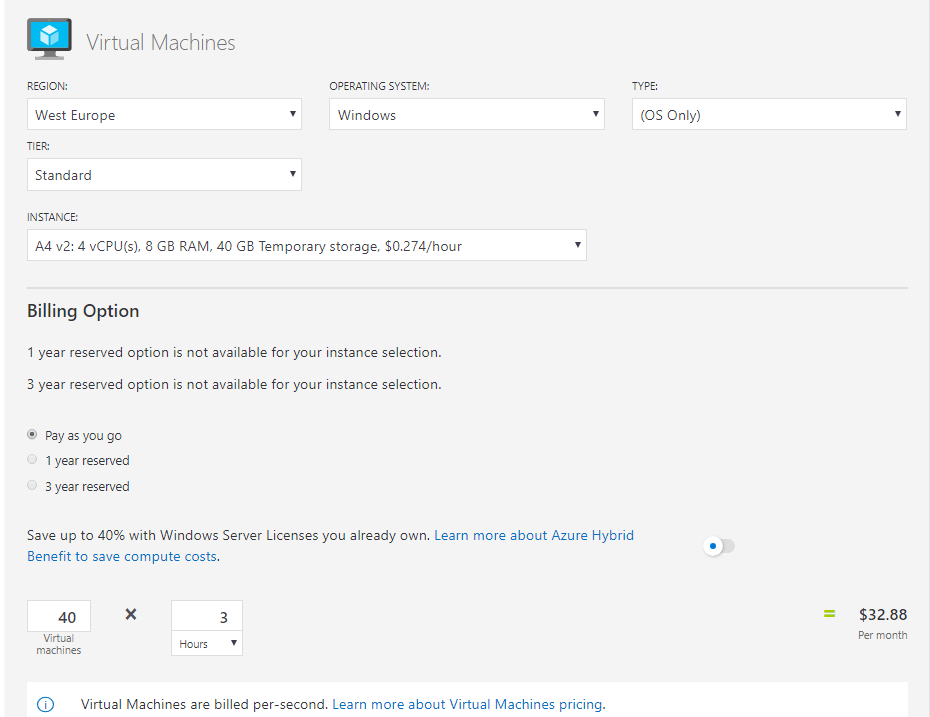
\includegraphics[width=\linewidth]{img/AzCalc.PNG}
	\caption{Screenshot van de Microsoft Azure Calculator. Hier kan je een kostenraming zien voor een computerexamen, voor één klas (40 studenten). Voor deze raming ben ik er vanuit gegaan dat de machines die aan de studenten gegeven worden over dezelfde systeemspecificaties beschikken als de huidige computers van Hogeschool Gent. Met deze configuratie zou een examen \$32.88 oftewel net geen 30 euro. Dit is de prijs zonder ondersteuning van Microsoft, en zonder de kost om een systeem met dergelijke virtualisatie op te zetten.}
	\label{fig:Calculator1}
\end{figure}

	
	
\newpage

\subsection{Beveiligde, configureerbare netwerkomgeving om internettoegang tot niet-toegestane sites vanop laptops tegen te gaan.	}

	\begin{figure}
	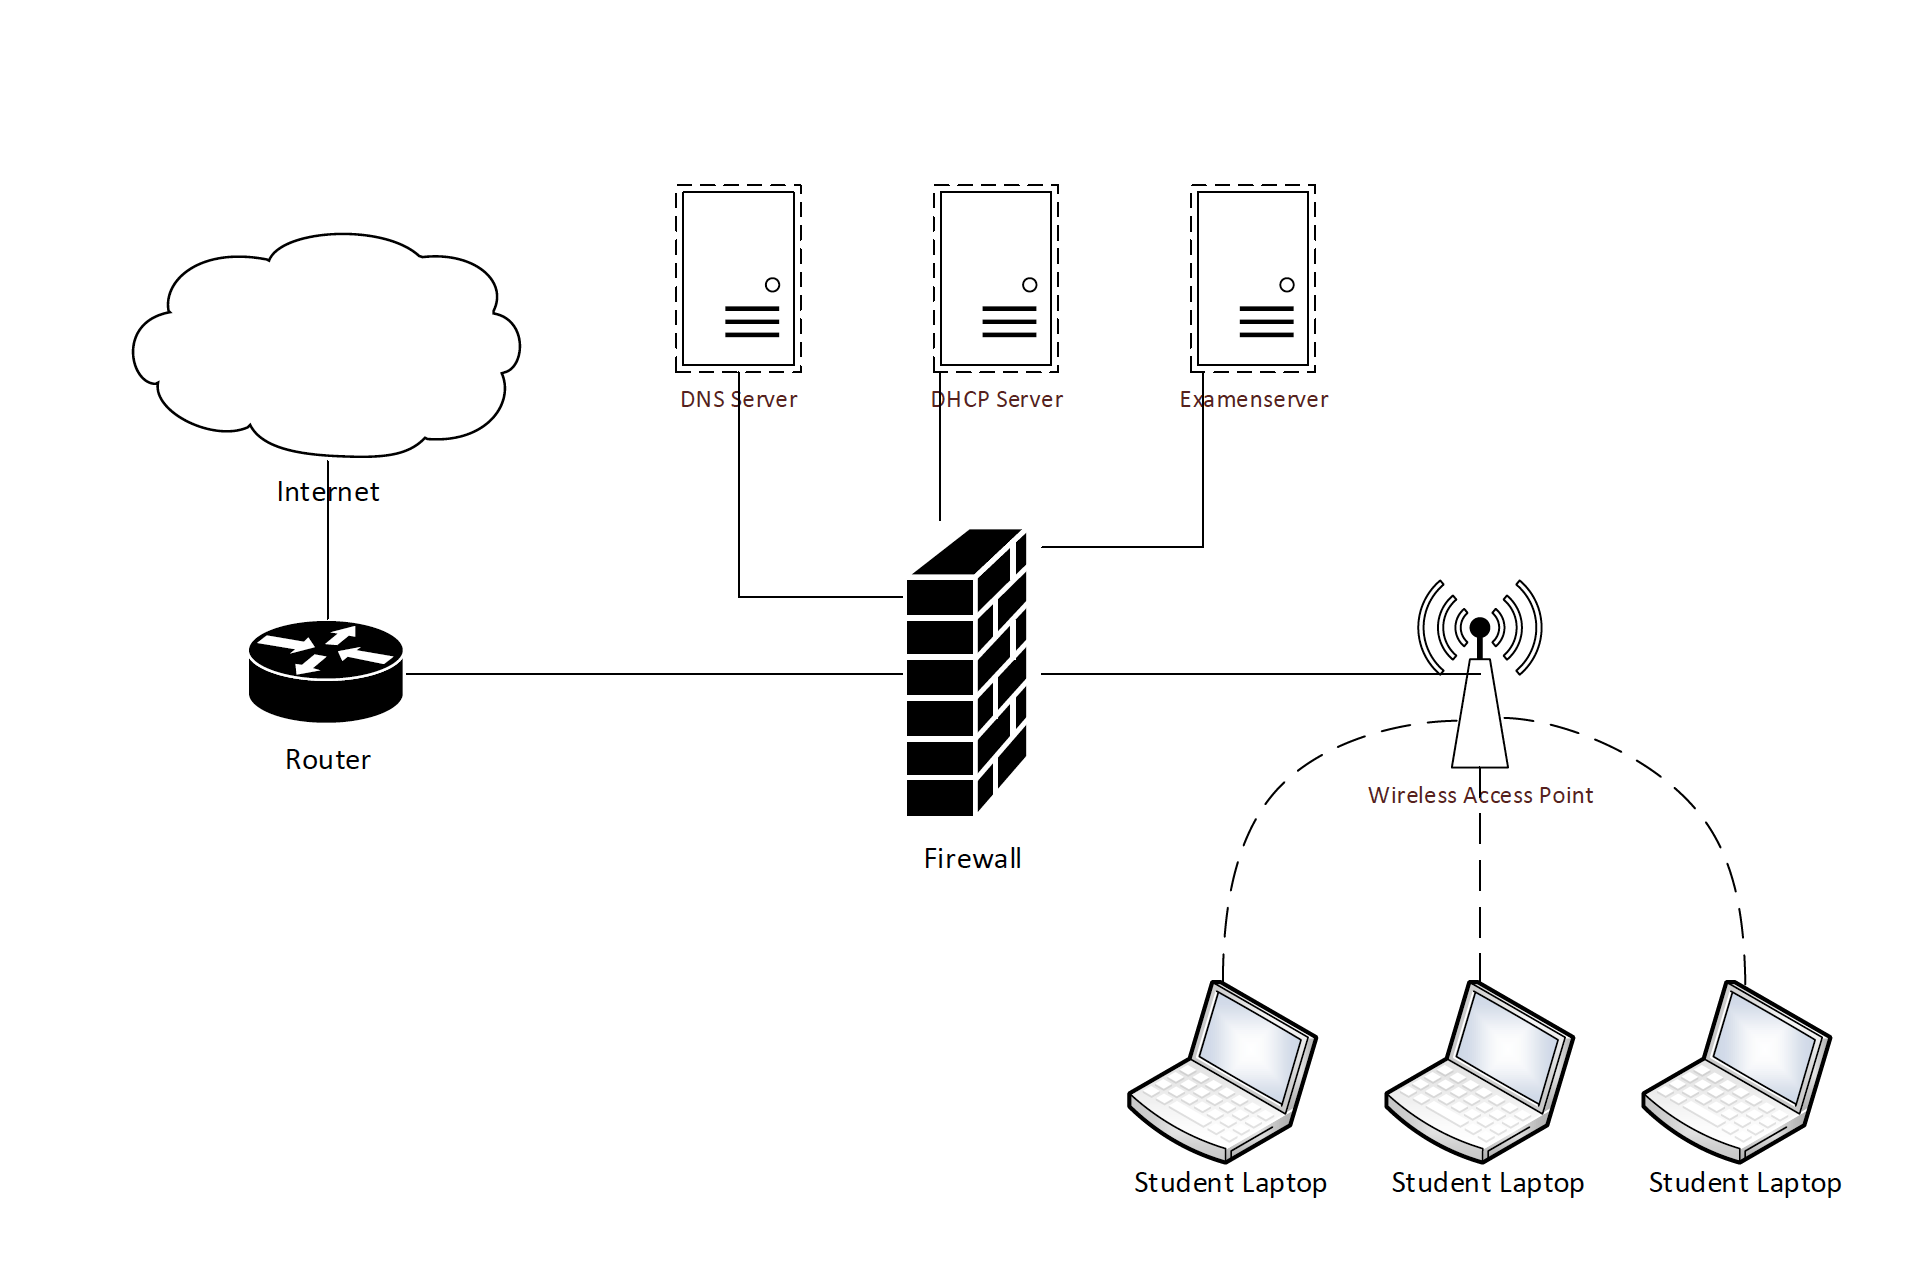
\includegraphics[width=\linewidth]{img/OpstellingNWOMG}
	\caption{Architectuurtekening van beveiligde netwerkomgeving (met lokale examenserver).}
	\label{fig:Omgeving1}
\end{figure}

\subsubsection{Omschrijving}
Dergelijke beveiligde omgeving kan snel opgezet en geconfigureerd worden voor een examen. Ze kan, bijvoorbeeld, bestaan uit:
\begin{itemize}
\item Een wireless Acces Point
\item Een router (Verbonden met het internet)
\item Een firewall
\item Een Ethernetswitch 
\item Een DNS server
\item Een DHCP server
\item Een examenserver (binnen of buiten het lokale netwerk)

\end{itemize}
Opmerking: dit hoeven geen 6 aparte servers/apparaten te zijn. Het wordt zo voorgesteld om duidelijker te zijn.

Concreet is het de bedoeling dat er met dit systeem voor elke student bij aanvang van elk examen een nieuwe single use login is, integratie met Microsoft Active Directory zou een meer effici\"{e}nte oplossing kunnen zijn hiervoor. Met deze kunnen ze verbinden met het netwerk via de wireless access point. Wanneer ze toegang tot het netwerk hebben kunnen ze het examen van de server halen (SFTP-server, Gitserver, webserver) en na het examen terug indienen. Dankzij de instellingen op de DNS server kunnen de studenten enkel aan websites waartoe ze toegang krijgen van de lectoren. Via de firewall wordt de verbinding met andere DNS servers of andere soorten servers ook geblokkeerd. Zo is het ook niet mogelijk voor studenten om de DNS server te omzeilen of om een VPN verbinding te maken en zo de controle te omzeilen. Er wordt ook concreet gemonitord of de student niet met een ander netwerk zou verbinden (Persoonlijke hotspot op GSM of HGSecure) door monitoring op de access point. De lectoren zullen een visuele controle moeten uitvoeren om te kijken of de student geen extra netwerkadaptor aangesloten heeft. 

Op deze manier ben je zeker dat een student geen fraude via het internet kan plegen, wanneer de omgeving juist geconfigureerd is.

Dit is niet de beste oplossing, zo kan je niet vermijden dat studenten documenten op hun eigen laptop kunnen bekijken. Volgens een lector van Hogeschool Gent is dit een tekortkoming van het nieuwe systeem. Een examen moet in de lijn liggen van de oefeningen die tijdens het jaar gemaakt zijn. Toegang tot onder andere die reeds gemaakte oefeningen tijdens het examen zou een te groot voordeel bieden, net zoals toegang tot theorie (indien dit niet toegestaan is), cheat-sheets of opgeloste vorige versies van examens. 




\section{GitHub Classroom}
\label{sec:GHC}

GitHub classroom is een product van GitHub. Het is hun oplossing voor code-management bij taken of examens. Momenteel wordt het reeds gebruikt voor projecten (Projecten III) en enkele vakken (Enterprise Linux, Onderzoekstechnieken) op Hogeschool Gent. Het zou perfect voor examens gebruikt kunnen worden, al moeten we er wel rekening mee houden dat er geen lokale GitHub classroom servers opgezet kunnen worden. Dit kan een breekpunt zijn voor security, omdat je over het publieke internet gevoelige documenten vestuurt. Maar wanneer dit op een correcte en veilige manier gebeurt (Via SSH of HTTPS), kunnen de meeste  gevaren die deze methode met zich meebrengt vermeden worden. 

Met GitHub classroom kan een lector de starterscode van een examen (bijvoorbeeld OOPII) in een repository plaatsen. Elke student kan dan een kopie binnenhalen bij de start van het examen en tijdens het examen na bepaalde mijlpalen committen om zo over back-ups en version control te beschikken. Bij elke commit kan er via CD/CI pipelines getest worden, bijvoorbeeld of de code compileert, of er in de code aan bepaalde vereisten voldaan werd (gebruik van commando's, compilatietijd e.d.). 

Met GitHub classroom zouden we het huidige systeem met Micorsoft Word, waarbij er code in een Word document geplakt wordt - om later afgedrukt en verbeterd te worden door een lector - veel effici\"{e}nter kunnen maken.  
\newpage 

\section{Conclusie}

Het enige BYOD Systeem uit deze selectie dat het onderzoeken waard is, is de beveiligde netwerkomgeving. Het voldoet niet aan alle vereisten, maar wel aan de meeste. Het biedt geen mogelijkheid tot controle over documenten, maar wel over internetgebruik en communicatie tussen studenten.

 Televic Avidanet Lite / AssessmentQ en Safe exam browser vielen al snel af omdat ze kiosk-software met zich meebrengen. Desktopvirtualisatie zonder een soort kiosk-software biedt helemaal geen veiligheid of controle. 


